\section{HARP extension for flexible performance-complexity balancing}\label{sec:our-method}

Graph representation learning methods such as node2vec typically have a large number of parameters -- on the widely used OGBN-ArXiv dataset (see \cite{hu_open_2021}), the state-of-the-art node2vec model has over 21 million parameters. At the same time, recent works in the domain of graph learning have started to focus more heavily on simpler methods as a competitive alternative to heavy-weight ones (see \cite{frasca_sign_2020,huang_combining_2020}). As the authors of \cite{chen_harp_2018} observed, HARP improves the performance of models when fewer labelled data are available. The proposed lower complexity models based on HARP could also improve performance in a setting where only low fidelity data are available for large parts of the graph. Coarser models could be trained on them, with a subsequent training of finer models using only a limited sample of high fidelity data.

In this work, we extend the general HARP framework to study the preformance-complexity characteristics of graph data. To this end, we propose alternatives to both the coarsening as well as the prolongation step of HARP. First, in Section~\ref{sec:adaptive-prolongation}, we replace the simple prolongation approach by an adaptive prolongation algorithm. Second, in Section~\ref{sec:coarsening-algorithms}, we study two alternative ways of coarsening the graph.

\subsection{Granularity of the HARP algorithm}

In standard HARP, once the coarsened graphs are obtained, the way to train the graph embedding is fairly straightforward. Starting with the coarsest graph, an embedding model such as node2vec is trained. Following that, a step to a graph that is one level finer is made. The embedding learned on the immediately preceding coarser graph is \name{prolonged} to the embedding of the following finer graph, in which the representations of merged nodes are copied and reused.
 Then, with this prolonged embedding as the starting state, the embedding algorithm continues training and this process is repeated until reaching the original graph.

While this style of prolongation is fine when HARP is used only as a means of pre-training, this approach is far too crude when studying the relationship between graph complexity and the quality of graph embedding and subsequent downstream applications. For example, the widely-used Cora dataset \cite{yang_revisiting_2016} has in its original form 2708 nodes, while the graph resulting from one application of the HARP coarsening schema has only about 1100 nodes (exact numbers may differ run-by-run). Such a relatively high reduction ratio effectively prevents any sufficient understanding of the relationship between graph reduction and changes in the quality of its embedding.

In order to offer a more fine-grained observation of the graph complexity and its effect on the downstream task, we present the adaptive prolongation approach. This algorithm works with the pre-coarsened graphs produced for example by HARP, however, the embedding is learned in a different manner.

\subsection{The adaptive prolongation approach}\label{sec:adaptive-prolongation}

\begin{figure}
  \centering
  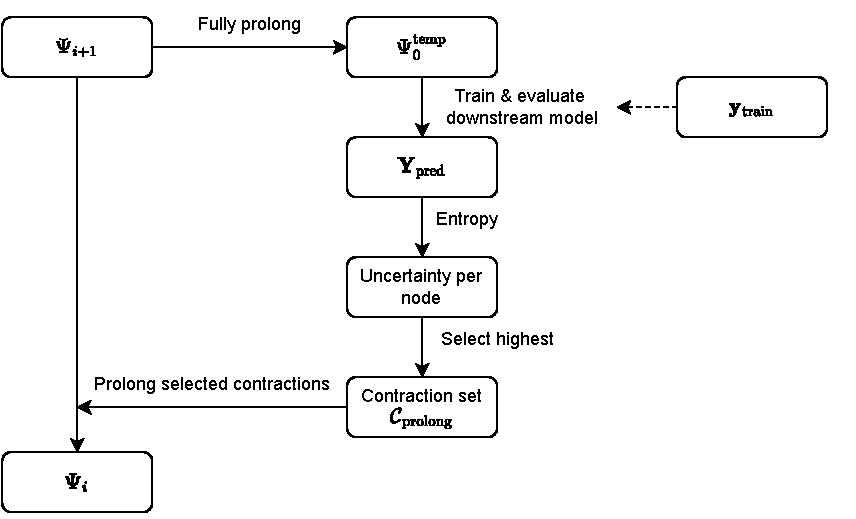
\includegraphics[width=\textwidth]{images/adaptive-prolongation/adaptive-prolongation.pdf}
    \caption{A schematic explanation of the adaptive prolongation algorithm for obtaining the embedding \( \Psi_{i} \) from \( \Psi_{i + 1} \).}
  \label{fig:adaptive-prolongation}
\end{figure}

The adaptive prolongation approach aims to replace the fixed steps defined by the used coarsening algorithm (such as HARP) by a variable number of smaller \enquote{micro-steps}, each of a predefined size that can be chosen independently from the underlying coarsening and its step size. Moreover, the prolongation procedure is driven by the interplay of the downstream task with the local properties of the underlying graph. This enables the method to produce embeddings with different level of granularity in different parts of the graph, e.g. an embedding that is coarse inside clusters of similar nodes and at the same time fine at the border between such clusters.

Let us denote \( \Psi_K, \dots, \Psi_0 \) the embedding sequence produced by the adaptive prolongation approach. To achieve the desired finer control over granularity the sequence \( \Psi_K, \dots, \Psi_0 \) needs to be decoupled from the graph sequence \( G_L, \dots, G_0 \), which in particular implies that the value of \( K \) is independent of \( L \). This is in contrast to the standard HARP prolongation, where the sequence of embeddings \( \Phi_{G_L}, \dots, \Phi_{G_0} \) is directly tied to the previously obtained graphs.

Similarly to standard HARP prolongation, the algorithm starts with the coarsest graph \( G_L \), trains a graph model to compute its embedding \( \Psi_K \) and gradually refines it until reaching the embedding \( \Psi_0 \) of \( G_0 \), or, alternatively, until a stopping criterion is met, as outlined in Section~\ref{sec:performance-complexity}. Instead of directly setting the value of \( K \), a fixed number of nodes \( n_p \) is prolonged in each step. These prolongation steps are interlaid with continued training of the graph model, as in standard HARP.  A description of a single prolongation step from \( \Psi_{i + 1} \) to \( \Psi_i \) follows, is schematically outlined in Figure~\ref{fig:adaptive-prolongation} and available as pseudocode in the supplementary material.

The procedure keeps track of all the edge contractions that were made in the dataset augmentation part of the algorithm and gradually reverses them. To this end, apart from the embedding \( \Psi_i \), the set of all contractions yet to be reversed as of step \( i \) is kept as \( \mathcal{C}_L^{(i)}, \dots, \mathcal{C}_0^{(i)} \), with the initial values \( \mathcal{C}_j^{(K)} \) corresponding to the underlying coarsening \( \varphi_j \) as defined in Section~\ref{sec:harp}.

In each prolongation step, the embedding \( \Psi_{i + 1} \) is prolonged to \( \Psi_i \) by selecting a set of \( n_p \) contractions \( \mathcal{C}_\mathrm{prolong} \) from the original coarsening procedure and undoing them by copying and reusing the embedding of the node resulting from the contraction to both of the nodes that were contracted. To obtain this set of contractions, nodes of \( G_0 \) are first ordered in such a way that corresponds to the usefulness of prolonging them. Subsequently, the set \( \mathcal{C}_\mathrm{prolong} \) is selected from \( \mathcal{C}_L^{(i + 1)}, \dots, \mathcal{C}_0^{(i + 1)} \) by selecting contractions affecting nodes in the aforementioned order, until \( n_p \) contractions are selected. If multiple contractions affecting the same node are available in the sequence \( \mathcal{C}_L^{(i + 1)}, \dots, \mathcal{C}_0^{(i + 1)} \), one is selected from \( \mathcal{C}_j^{(i + 1)} \) corresponding to the coarsest-level coarsening, that is, from \( \mathcal{C}_j^{(i + 1)} \) with the highest possible \( j \). The sequence \( \mathcal{C}_L^{(i)}, \dots, \mathcal{C}_0^{(i)} \) is produced from \( \mathcal{C}_L^{(i + 1)}, \dots, \mathcal{C}_0^{(i + 1)} \) by removing all of the edges contained in \( \mathcal{C}_\mathrm{prolong} \) (each edge from \( \mathcal{C}_\mathrm{prolong} \) will be contained in exactly one of \( \mathcal{C}_L^{(i + 1)}, \dots, \mathcal{C}_0^{(i + 1)} \)).

To obtain an ordering of nodes of \( G_0 \) based on the usefulness of their prolongation, the embedding \( \Psi_{i + 1} \) is fully prolonged to a temporary embedding of the full graph, \( \Psi_0^\mathrm{temp} \). A downstream model is then trained using this temporary embedding to obtain \( \mathmat{Y}_\mathrm{pred} \), the predicted posterior distribution of classes for each node in \( G_0 \) (e.g. the output of the softmax layer of an MLP). The entropy of this distribution is measured, representing the amount of uncertainty in the classifier for each given node. The nodes are ordered based on the entropy from highest to lowest. This reflects the principle that it is most useful to prolong those nodes where the downstream classifier is the least certain. For downstream tasks other than node classification, the ordering would need to be defined in a different manner (for example using labels, which are not available for all nodes in our case), however the approach of prolonging the nodes about which the downstream model is the most uncertain can be extended to other tasks.

\subsection{More general approaches to coarsening}\label{sec:coarsening-algorithms}

While the adaptive prolongation approach substantially generalizes the original method into a powerful tool for studying and leveraging graph structure and its properties under a coarsening, it still relies on the pre-computed coarsenings to guide the prolongation process. In this section, we first present a brief overview of the coarsening algorithm as proposed by \cite{chen_harp_2018}, followed by two alternative proposals for coarsening construction based on graph diffusion.

\subsubsection{HARP coarsening}\label{sec:harp-coarsening}

The authors of \cite{chen_harp_2018} introduce two particular coarsening methods that together realize the function \( \varphi_i \) from Section~\ref{sec:harp} -- \name{edge collapsing} and \name{star collapsing}. Edge collapsing is a very simple method -- out of all the edges \( E \left( G \right) \), a maximal subset \( E' \) is selected randomly such that no two edges from \( E' \) are incident on the same node. Then, each edge in \( E' \) is contracted. Such an algorithm on its own is not sufficient to coarsen star-like structures with a high-degreen \textit{hub} node. To coarsen such structures effectively, the star collapsing algorithm pairwise merges the neighbours of such hub nodes, taking them in the order of decreasing node degree and never merging one node twice.

These two approaches are combined in the original HARP method, with each coarsening step being a star collapsing step followed by an edge collapsing step. Of a particular note is the fact that such a coarsening scheme cannot be constructed as a subset of edges of the graph. The star collapsing algorithm merges nodes that are adjacent to a common hub node, however, these nodes need not be connected by an edge. However, in our previously published work, we experimentally verified that the star collapsing algorithm can be replaced by a similar algorithm that repeatedly merges nodes adjacent on a hub node with the hub node itself.

\subsubsection{Graph diffusion coarsening}\label{sec:gdc-coarsening}

Our definition of a graph coarsening requires choosing some edges from the original graph. Intuitively, one way of constructing a graph coarsening would be to merge nodes which are similar and therefore no significant amount of information is lost due to such a coarsening. Following both of these premises, we propose a coarsening based on Graph Diffusion Convolution (GDC) \cite{gasteiger_diffusion_2019} algorithm. GDC is a general graph transformation which, in an overview, constructs for a given graph a new edge set, represented by a so-called sparsified generalized graph diffusion matrix \( \hat{\mathmat{S}} \), which would, in the original setting of the method, be used as a replacement for the adjacency matrix of the graph. To apply this algorithm as a way of coarsening the graph, the edge set obtained by GDC is intersected with the edges of the original graph and the resulting edges contracted in the graph, i.e.,
\[ \mathcal{C} = E \left( G_{\hat{\mathmat{S}}} \right) \cap E \left( G \right), \]
using the construction of a graph coarsening as a subset of its edges, as presented in Section~\ref{sec:harp}.

In principle, the authors of GDC define the generalized graph diffusion matrix
\begin{equation}\label{eq:gdc-matrix}
    \mathmat{S} = \sum_{k = 1}^\infty \theta_k \mathmat{T}^k
\end{equation}
such that the power series converges. The parameters \( \theta_k \) together with the generalized transition matrix \( \mathmat{T} \) define the exact way in which the diffusion is achieved. Among the choices for \( \mathmat{T} \) is the random walk transition matrix \( \mathmat{T}_ \mathrm{rw} = \mathmat{A} \mathmat{D}^{-1} \) and the symmetric transition matrix \( \mathmat{T}_\mathrm{sym} = \mathmat{D}^{-\frac{1}{2}} \mathmat{A} \mathmat{D}^{-\frac{1}{2}} \) where \( \mathmat{D} \) is the diagonal matrix of node degrees. Two special cases of this general schema using the random walk transition matrix are the Personalized PageRank algorithm (PPR) \cite{page_pagerank_1999} and the heat kernel \cite{kondor_diffusion_2002}.

Graph sparsification needs to be used in order to preserve reasonable computational requirements throughout the diffusion. In GDC, two such methods are considered -- thresholding the matrix values and selecting top-\( k \) entries for each column of the matrix. In any case, the matrix is normalized after sparsification, thus finally producing \( \hat{\mathmat{S}} \).
